\documentclass{standalone}
\usepackage{tikz}
\usetikzlibrary{patterns, positioning}
\usepackage[sfdefault]{ClearSans} %% option 'sfdefault' activates Clear Sans as the default text font
\usepackage[T1]{fontenc}

\begin{document}
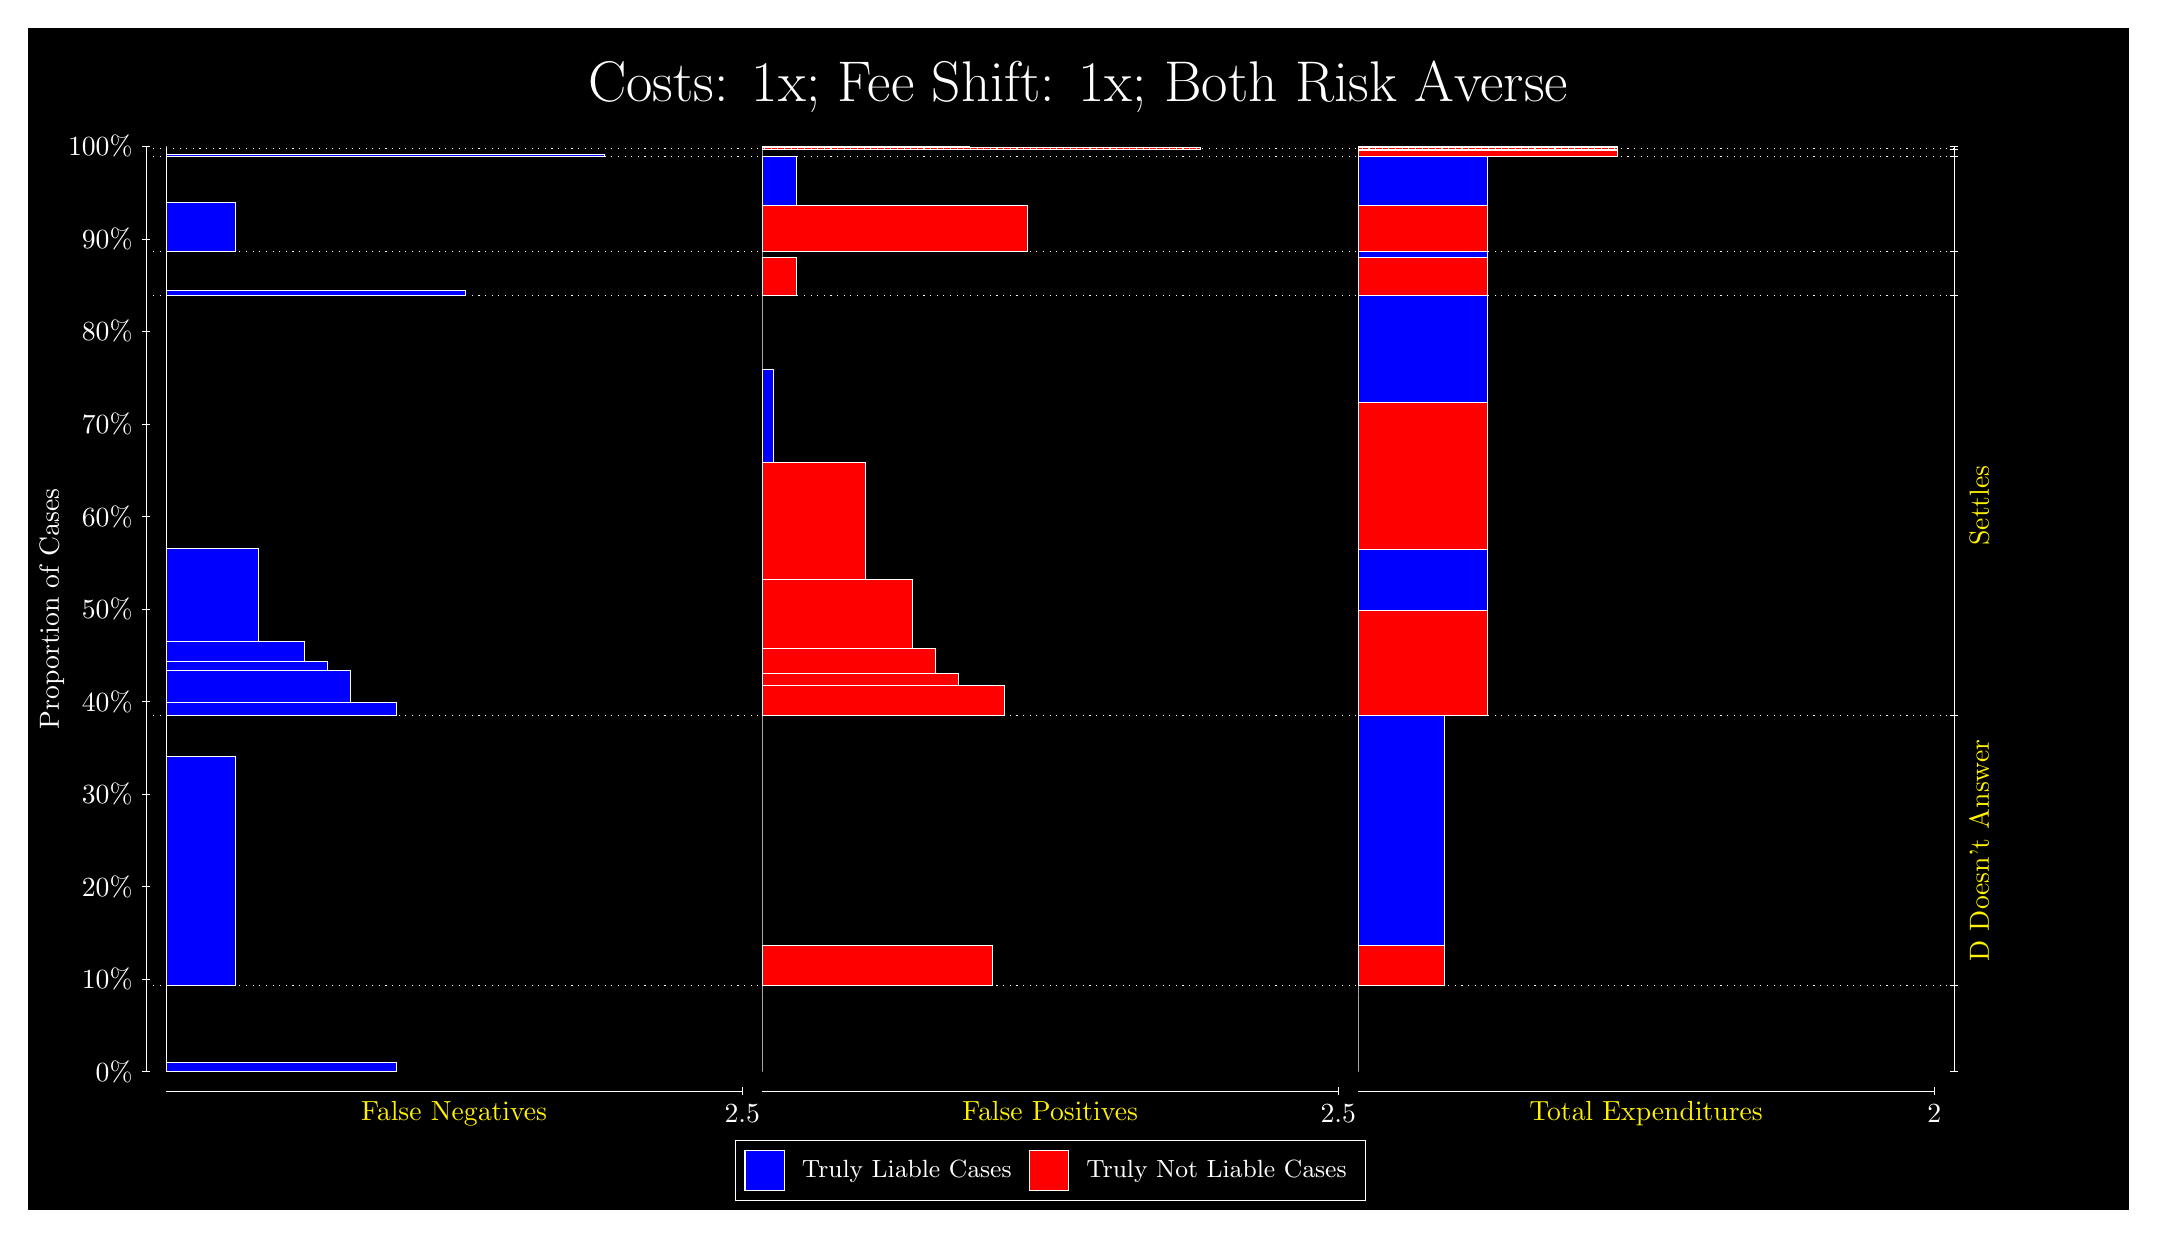
\begin{tikzpicture}
\draw[fill=black] (0,0) rectangle (26.667,15);
\draw[text=white] (0,13.5) rectangle (26.667,15) node[midway] {\huge Costs: 1x; Fee Shift: 1x; Both Risk Averse};
\draw[white, very thin] (1.5,1.75) -- (1.5,13.5);
\node[rotate=90, text=white, anchor=center] at (0.3, 7.625) {Proportion of Cases};
\draw[white, very thin] (1.45,1.75) -- (1.55,1.75);
\node[text=white, anchor=east] at (1.45, 1.75) {0\%};
\draw[white, very thin] (1.45,2.925) -- (1.55,2.925);
\node[text=white, anchor=east] at (1.45, 2.925) {10\%};
\draw[white, very thin] (1.45,4.1) -- (1.55,4.1);
\node[text=white, anchor=east] at (1.45, 4.1) {20\%};
\draw[white, very thin] (1.45,5.275) -- (1.55,5.275);
\node[text=white, anchor=east] at (1.45, 5.275) {30\%};
\draw[white, very thin] (1.45,6.45) -- (1.55,6.45);
\node[text=white, anchor=east] at (1.45, 6.45) {40\%};
\draw[white, very thin] (1.45,7.625) -- (1.55,7.625);
\node[text=white, anchor=east] at (1.45, 7.625) {50\%};
\draw[white, very thin] (1.45,8.8) -- (1.55,8.8);
\node[text=white, anchor=east] at (1.45, 8.8) {60\%};
\draw[white, very thin] (1.45,9.975) -- (1.55,9.975);
\node[text=white, anchor=east] at (1.45, 9.975) {70\%};
\draw[white, very thin] (1.45,11.15) -- (1.55,11.15);
\node[text=white, anchor=east] at (1.45, 11.15) {80\%};
\draw[white, very thin] (1.45,12.325) -- (1.55,12.325);
\node[text=white, anchor=east] at (1.45, 12.325) {90\%};
\draw[white, very thin] (1.45,13.5) -- (1.55,13.5);
\node[text=white, anchor=east] at (1.45, 13.5) {100\%};

\draw[white, very thin] (24.457,1.75) -- (24.457,13.5);
\draw[white, very thin] (24.407,1.75) -- (24.507,1.75);
\node[anchor=west] at (24.407, 1.75) {};
\draw[white, very thin] (24.407,2.8432) -- (24.507,2.8432);
\node[anchor=west] at (24.407, 2.8432) {};
\draw[white, very thin] (24.407,6.2692) -- (24.507,6.2692);
\node[anchor=west] at (24.407, 6.2692) {};
\draw[white, very thin] (24.407,11.607) -- (24.507,11.607);
\node[anchor=west] at (24.407, 11.607) {};
\draw[white, very thin] (24.407,12.163) -- (24.507,12.163);
\node[anchor=west] at (24.407, 12.163) {};
\draw[white, very thin] (24.407,13.375) -- (24.507,13.375);
\node[anchor=west] at (24.407, 13.375) {};
\draw[white, very thin] (24.407,13.467) -- (24.507,13.467);
\node[anchor=west] at (24.407, 13.467) {};
\draw[white, very thin] (24.407,13.5) -- (24.507,13.5);
\node[anchor=west] at (24.407, 13.5) {};

\draw[white, very thin, fill=blue] (1.75,1.75) rectangle (4.6775,1.865);
\draw[white, very thin, fill=red] (1.75,1.865) rectangle (1.75,2.8432);
\draw[white, very thin, fill=blue] (1.75,2.8432) rectangle (2.6283,5.7552);
\draw[white, very thin, fill=red] (1.75,5.7552) rectangle (1.75,6.2692);
\draw[white, very thin, fill=blue] (1.75,6.2692) rectangle (4.6775,6.4455);
\draw[white, very thin, fill=blue] (1.75,6.4455) rectangle (4.092,6.8465);
\draw[white, very thin, fill=blue] (1.75,6.8465) rectangle (3.7993,6.9578);
\draw[white, very thin, fill=blue] (1.75,6.9578) rectangle (3.5065,7.2087);
\draw[white, very thin, fill=blue] (1.75,7.2087) rectangle (2.921,8.3895);
\draw[white, very thin, fill=red] (1.75,8.3895) rectangle (1.75,11.607);
\draw[white, very thin, fill=blue] (1.75,11.607) rectangle (5.5558,11.674);
\draw[white, very thin, fill=red] (1.75,11.674) rectangle (1.75,12.163);
\draw[white, very thin, fill=blue] (1.75,12.163) rectangle (2.6283,12.791);
\draw[white, very thin, fill=red] (1.75,12.791) rectangle (1.75,13.375);
\draw[white, very thin, fill=blue] (1.75,13.375) rectangle (7.3123,13.393);
\draw[white, very thin, fill=red] (1.75,13.393) rectangle (1.75,13.467);
\draw[white, very thin, fill=red] (1.75,13.467) rectangle (1.75,13.485);
\draw[white, very thin, fill=blue] (1.75,13.485) rectangle (1.75,13.5);
\draw[white, very thin, fill=red] (9.3189,1.75) rectangle (9.3189,2.7282);
\draw[white, very thin, fill=blue] (9.3189,2.7282) rectangle (9.3189,2.8432);
\draw[white, very thin, fill=red] (9.3189,2.8432) rectangle (12.246,3.3571);
\draw[white, very thin, fill=blue] (9.3189,3.3571) rectangle (9.3189,6.2692);
\draw[white, very thin, fill=red] (9.3189,6.2692) rectangle (12.393,6.6569);
\draw[white, very thin, fill=red] (9.3189,6.6569) rectangle (11.807,6.8052);
\draw[white, very thin, fill=red] (9.3189,6.8052) rectangle (11.515,7.1241);
\draw[white, very thin, fill=red] (9.3189,7.1241) rectangle (11.222,8.001);
\draw[white, very thin, fill=red] (9.3189,8.001) rectangle (10.636,9.4866);
\draw[white, very thin, fill=blue] (9.3189,9.4866) rectangle (9.4652,10.667);
\draw[white, very thin, fill=blue] (9.3189,10.667) rectangle (9.3189,11.607);
\draw[white, very thin, fill=red] (9.3189,11.607) rectangle (9.758,12.096);
\draw[white, very thin, fill=blue] (9.3189,12.096) rectangle (9.3189,12.163);
\draw[white, very thin, fill=red] (9.3189,12.163) rectangle (12.686,12.747);
\draw[white, very thin, fill=blue] (9.3189,12.747) rectangle (9.758,13.375);
\draw[white, very thin, fill=red] (9.3189,13.375) rectangle (9.3189,13.45);
\draw[white, very thin, fill=blue] (9.3189,13.45) rectangle (9.3189,13.467);
\draw[white, very thin, fill=red] (9.3189,13.467) rectangle (14.881,13.485);
\draw[white, very thin, fill=blue] (9.3189,13.485) rectangle (11.954,13.5);
\draw[white, very thin, fill=red] (16.888,1.75) rectangle (16.888,2.7282);
\draw[white, very thin, fill=blue] (16.888,2.7282) rectangle (16.888,2.8432);
\draw[white, very thin, fill=red] (16.888,2.8432) rectangle (17.986,3.3571);
\draw[white, very thin, fill=blue] (16.888,3.3571) rectangle (17.986,6.2692);
\draw[white, very thin, fill=red] (16.888,6.2692) rectangle (18.534,7.6133);
\draw[white, very thin, fill=blue] (16.888,7.6133) rectangle (18.534,8.3766);
\draw[white, very thin, fill=red] (16.888,8.3766) rectangle (18.534,10.25);
\draw[white, very thin, fill=blue] (16.888,10.25) rectangle (18.534,11.607);
\draw[white, very thin, fill=red] (16.888,11.607) rectangle (18.534,12.096);
\draw[white, very thin, fill=blue] (16.888,12.096) rectangle (18.534,12.163);
\draw[white, very thin, fill=red] (16.888,12.163) rectangle (18.534,12.747);
\draw[white, very thin, fill=blue] (16.888,12.747) rectangle (18.534,13.375);
\draw[white, very thin, fill=red] (16.888,13.375) rectangle (20.181,13.45);
\draw[white, very thin, fill=blue] (16.888,13.45) rectangle (20.181,13.467);
\draw[white, very thin, fill=red] (16.888,13.467) rectangle (20.181,13.485);
\draw[white, very thin, fill=blue] (16.888,13.485) rectangle (20.181,13.5);
\draw[white, dotted] (1.5,2.8432) -- (24.457,2.8432);
\draw[white, dotted] (1.5,6.2692) -- (24.457,6.2692);
\draw[white, dotted] (1.5,11.607) -- (24.457,11.607);
\draw[white, dotted] (1.5,12.163) -- (24.457,12.163);
\draw[white, dotted] (1.5,13.375) -- (24.457,13.375);
\draw[white, dotted] (1.5,13.467) -- (24.457,13.467);
\draw[white, very thin] (1.75,1.5) -- (9.0689,1.5);
\node[text=yellow, anchor=north] at (5.4094, 1.5) {False Negatives};
\draw[white, very thin] (9.0689,1.45) -- (9.0689,1.55);
\node[text=white, anchor=north] at (9.0689, 1.45) {2.5};

\draw[white, very thin] (9.3189,1.5) -- (16.638,1.5);
\node[text=yellow, anchor=north] at (12.978, 1.5) {False Positives};
\draw[white, very thin] (16.638,1.45) -- (16.638,1.55);
\node[text=white, anchor=north] at (16.638, 1.45) {2.5};

\draw[white, very thin] (16.888,1.5) -- (24.207,1.5);
\node[text=yellow, anchor=north] at (20.547, 1.5) {Total Expenditures};
\draw[white, very thin] (24.207,1.45) -- (24.207,1.55);
\node[text=white, anchor=north] at (24.207, 1.45) {2};


\node[text=yellow, centered, rotate=90] at (24.777, 4.5562) {D Doesn't Answer};
\node[text=yellow, centered, rotate=90] at (24.777, 8.938) {Settles};





\draw (12.978300999999998,1.5) node[draw=none] (baseCoordinate) {};
\begin{scope}[align=center]
        \matrix[scale=0.5, draw=white, below=0.5cm of baseCoordinate, nodes={draw}, column sep=0.1cm]{
            \node[rectangle, draw, minimum width=0.5cm, minimum height=0.5cm, fill=blue] {}; &
            \node[draw=none, font=\small, text=white] (B) {Truly Liable Cases}; &
            \node[rectangle, draw, minimum width=0.5cm, minimum height=0.5cm, fill=red] {}; &
            \node[draw=none, font=\small, text=white] (B) {Truly Not Liable Cases}; \\
            };
\end{scope}

\end{tikzpicture}
\end{document}